% Chapter Template

\chapter{Fluorescence intensity classification} % Main chapter title

\label{Chapter5} % Change X to a consecutive number; for referencing this chapter elsewhere, use \ref{ChapterX}


%----------------------------------------------------------------------------------------
%	INTRODUCTION
%----------------------------------------------------------------------------------------

The fluorescence intensity is a parameter that describes the \textit{clarity} of cells in an image. It is a subjective parameter which, unfortunately, doesn't have a strong theoretical explanation. The fluorescence intensity is described with three values - positive, intermediate and negative. The positive value defines images in which cells are perfectly separated from the background, while the negative value defines images in which cells  cannot be identified. The intermediate value covers images that are nor positive nor negative. This parameter is used as a symbolic feature later in the process, but for the sake of \textit{standard procedure} it is estimated separately. \\


In \cite{Rigon2007} Rigon studied the variability of decisions made by doctors and showed that it is difficult to achieve a consensus about unique determination of the fluorescence intensity value. The lack of the underlying model is making this problem hard to formulate. The intuition behind the suggested approach is an assumption that the intensity level could be observed in the histogram of an image. The fluorescence intensity should correspond to the difference of a region describing the background and a region describing cells. Following the intuition, the image histogram is approximated with the Gaussian mixture model. \\

The idea is to approximate the histogram with a mixture of two Gaussian functions - one representing the background and second one to model the cells. The intuition is that images with positive intensity should have Gaussians with higher means and more further apart. 


%-----------------------------------------------------------------------------------------
%     Classifying intensity
%-----------------------------------------------------------------------------------------

\section{Classifying intensity}

Once the histogram has been approximated with two Gaussian functions, the estimated means and variances has been taken as features for the classification. A \textit{support vector machine} with \textit{radial basis functions} as kernel function has been trained for the task. Evaluation is performed using a 10-fold cross validation. \\



%--------------------------------------------------%
%                                                  %
%               SVM                                %
%                                                  %
%--------------------------------------------------%


\subsection{Support Vector Machine}


The Support vector machine is a very popular machine learning technique. It is a representative of a more general class of \textit{kernel methods}. The most interesting property of the support vector machine is that it tries to find the \textit{optimal hyperplane} that separates classes. Consider a two-class case. The sample is $\mathcal{D} = \{ \mathbf{x}^{(i)}, y^{(i)} \}_{i=1}^N$ where $y^{(i)} = 1$ if $\mathbf{x}^{(i)} \in \mathcal{C}_1$ and $y^{(i)} = -1$ if $\mathbf{x}^{(i)} \in \mathcal{C}_2$. We want to find a margin $\mathbf{w}$ so that

\begin{equation*}
	\mathbf{w}^T\mathbf{x}^{(i)} + w_o \geq +1 \quad \mathtt{for} \quad y^{(i)} = 1
\end{equation*}

\begin{equation*}
	\mathbf{w}^T\mathbf{x}^{(i)} + w_o \leq -1 \quad \mathtt{for} \quad y^{(i)} = -1
\end{equation*}

or simplified 

\begin{equation*}
	y^{(i)}(\mathbf{w}^T\mathbf{x}^{(i)} + w_0) \geq 1.
\end{equation*}

The support vector machine extends the \textit{basic} hyperplane requirement - setting the instances on the right side of the hyperplane - by trying to maximize the margin - the distance from the hyperplane to the instances closest to it. So, the \textit{optimal separating hyperplane} is the one that maximizes the margin. \\

The distance of $\mathbf{x}^{(i)}$ to the hyperplane equals to 

\begin{equation}
	\frac{ | \mathbf{w}^T\mathbf{x}^{(i)} - w_0 | }{ \Vert \mathbf{w} \Vert}.
\end{equation}

Finding the maximal margin can be expressed as

\begin{equation}
	\frac{y^{(i)}(\mathbf{w}^T\mathbf{x} - w_0)}{\Vert \mathbf{w} \Vert} \geq \rho, \forall i,
\end{equation}

i.e., we want the margin to be at least $\rho$. As there are infinitely many solutions that can be obtained by scaling $\mathbf{w}$, we fix the $\rho \Vert \mathbf{w} \Vert = 1$ and minimize $\Vert \mathbf{w} \Vert$ to maximize the margin. The problem can now be written in a form of quadratic optimization problem

\begin{align*}
	\min_{\mathbf{w}, w_0} & \quad \frac{1}{2} \Vert \mathbf{w} \Vert \\
	\mathtt{subject \ to} & \quad  y^{(i)} \left ( \mathbf{w}^T\mathbf{x} + w_0  \right ) \geq 1.
\end{align*}

Now there will be instances that are $\frac{1}{\Vert \mathbf{w} \Vert}$ away from the hyperplane and the total margin equals to $\frac{2}{\Vert \mathbf{w} \Vert}$. \\

If the problem is not linearly separable, one trick is to map the problem to a new space, with more dimension that the original space, by using nonlinear basis functions. It is generally the case that higher dimensional representation is easier to separate. One of those mapping functions are \textit{radial basis functions}. 


%---------------------------------------%
%                                       %
%                RBF                    %
%                                       %
%---------------------------------------%
 
\subsection{Radial basis functions}

Radial basis functions are an instance of a \textit{local representation}, where for a given input, only a few factors are \textit{active}. It is in a way a partition of space so that \textit{locally tuned} partitions are selective to only certain inputs. \\

With the concept of local partitioning we need to define a measure of similarity between an input $\mathbf{x}^{(i)}$ and local clusters $\boldsymbol \mu^1, \ldots, \boldsymbol \mu^n$. Radial basis functions are defined as

\begin{equation}
	\mathbf{r}(\mathbf{x}^{(i)}, \boldsymbol \mu^k) = exp \left (- \frac{\Vert \mathbf{x}^{(i)}  - \boldsymbol \mu^k \Vert}{2\sigma_k^2} \right ),
\end{equation} 

that is, it uses the Euclidean distance as a measure of similarity and Gaussian function as a response function. The response function express a property of having a maximum where $\mathbf{x}^{(i)} = \boldsymbol \mu^k$ and decreasing as they get less similar. 




%--------------------------------------%
%                                      %
%           EVALUATION                 %
%                                      %
%--------------------------------------%

\subsection{Results}

One issue that might occur is a bad estimation of the background or cell body as some cells takes a very small portion of an image or, on the other hand, takes almost a whole image when segmented as shown in image \ref{fig:Bad}. To see how this influences the problem, histograms are approximated with Gaussian functions in two ways. First, the histogram is as in Chapter \ref{Chapter4}, without any restrictions. Second, the background and cells part of an image are separated and each part is approximated with a Gaussian individually. \\

\begin{figure}
	\begin{minipage}[h]{0.32\linewidth}
		\begin{flushright}
			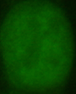
\includegraphics[height=2cm]{Figures/intensity/image1}
		\end{flushright}
	\end{minipage}
	\begin{minipage}[h]{0.32\linewidth}
		\centering
		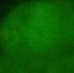
\includegraphics[height=2cm]{Figures/intensity/image2}
	\end{minipage}
	\begin{minipage}[h]{0.32\linewidth}
		\begin{flushleft}
			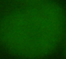
\includegraphics[height=2cm]{Figures/intensity/image3}
		\end{flushleft}
	\end{minipage}
	\caption{Potential image that could obtain bad estimation}
	\label{fig:Bad}
\end{figure}

Table \ref{res:SepReg} summarizes the results obtained with separation of background and cell regions (a) and without (b). The accuracy of the proposed solution is 96.21 \% and 96.08 \% for separation and without it, respectively. As the results for both cases don't show any significant difference, the stability of the method is promising.  The best performance reported so far is 92,6 \% although the authors have used a private data set that is not available online, so it is hard to make a comparison.  So far, the results of this data set are not yet reported. \\

So far, the evaluation has been performed on  cell level - the intensity level is estimated on cell level. In practice, the intensity level is assigned on the image level, which means that every cell in an image is assigned to the same value of the parameter, regardless of the variations of a specific subset of cells. The intensity level of an image is then determined by averaging the assigned intensity levels of the cells on the image. With that approach, a 100 \% accuracy is achieved.




\begin{table}
	\caption{Results of intensity classification}
	\label{res:SepReg}
	\begin{minipage}[h]{0.49\linewidth}
		\begin{center}
			\begin{tabular}{c c| c c}
				 & & \multicolumn{2}{c}{True} \\
			     & & \textbf{pos} & \textbf{int} \\
			    \hline
			    \multirow{2}{*}{\rotatebox[origin=c]{90}{Pred}} & \textbf{pos} & \cellcolor{gray}96.98 \% & 4.96 \% \\
			    & \textbf{int} & 3.02 \% & \cellcolor{gray}95.04 \%
			\end{tabular} \\
		a)
		\end{center}
	\end{minipage}
	\begin{minipage}[h]{0.49\linewidth}
		\begin{center}
			\begin{tabular}{c c| c c}
				 & & \multicolumn{2}{c}{True} \\
			     & & \textbf{pos} & \textbf{int} \\
			    \hline
			    \multirow{2}{*}{\rotatebox[origin=c]{90}{Pred}} & \textbf{pos} & \cellcolor{gray}96.50 \% & 5.76 \% \\
			    & \textbf{int} & 3.50 \% & \cellcolor{gray}94.24 \%
			\end{tabular} \\
			b)
		\end{center}
	\end{minipage}
\end{table}

